\documentclass[11pt]{beamer}
\usetheme{Warsaw}
\usepackage[utf8]{inputenc}
\usepackage[spanish]{babel}
\usepackage{amsmath}
\usepackage{amsfonts}
\usepackage{amssymb}
\usepackage{graphicx}
\author{N.Pérez-Medina}
\title{Capítulo 4 - Determinismo y predictibilidad.}
\setbeamercovered{transparent} 
\setbeamertemplate{navigation symbols}{} 
\logo{
\includegraphics[scale=0.04]{logo_fing_uach_bn.png} } 
\institute{\textbf{FING - UACH}
	\\
	\begin{small}
	\textit{Resumen del libro 'Análisis de series de tiempo no lineales' de Kantz y Schreiber}\\
	\end{small}
	
	\bigskip
	
	\begin{small}
	\textbf{Catedrático:} Dr. José Luis Herrera Aguilar
	\end{small}		
	} 
\date{\today} 
\subject{Series de tiempo} 


% Para tener un morado coqueto
\definecolor{lightPurple}{RGB}{186, 146, 209} % Morado claro
\definecolor{darkPurple}{RGB}{98, 54, 150}    % Morado oscuro
\setbeamercolor{structure}{fg=darkPurple} % Color principal para estructuras
\setbeamercolor{frametitle}{bg=darkPurple, fg=white} % Título del marco
\setbeamercolor{block title}{bg=darkPurple, fg=white} % Título de bloques
\setbeamercolor{block body}{bg=lightPurple!30, fg=black} % Cuerpo de bloques

\begin{document}

\begin{frame}
\maketitle
\end{frame}

\begin{frame}
\tableofcontents
\end{frame}

\section{Fuentes de predictibilidad}
\begin{frame} 
\tableofcontents[currentsection] % Solo muestra la sección actual
\end{frame}

\begin{frame}{Noción de predictibilidad}
\begin{block}{En general}
Un argumento convincente para la existencia de un patrón es si puede usarse para dar una mejor predicción.
\end{block}
\centering
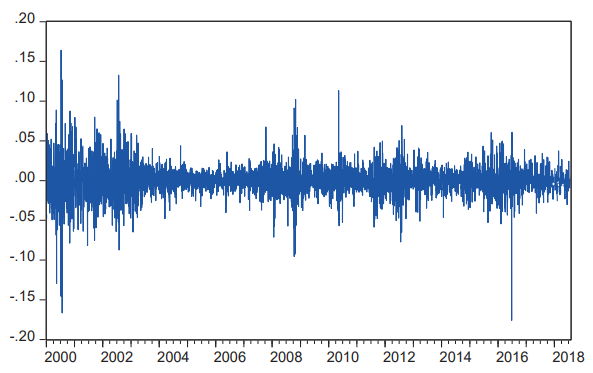
\includegraphics[scale=0.4]{idea-grafica.png} 
\end{frame}

\begin{frame}{Señales conocidas}
\small
\begin{block}{Si una señal...}
\begin{itemize}
\item \textbf{No cambia o cambia poco} -> La última observación es pronóstico perfecto para la siguiente
\item \textbf{Cambia periódicamente} -> Cuestión de observar un ciclo completo
\item \textbf{Cambia aleatoriamente} -> La mejor predicción es el valor medio
\end{itemize}
\end{block}
\end{frame}

\begin{frame}{Señales que estudiaremos}
\begin{block}{}
Señales que NO son \textit{periódicas} pero contienen algún tipo de \textit{\textbf{estructura}} que puede aprovecharse para obtener mejores predicciones.
\end{block}
\end{frame}

\begin{frame}{Error cuadrático medio}
Es una manera de cuantificar el éxito de las predicciones que hacemos.
\begin{block}{$rms$}
Si predecimos el resultado de las mediciones en los tiempos $n$ como $\hat{s}_n$, mientras que las mediciones reales son $s_n$, entonces el error $rms$ de predicción es
\begin{equation}
e = \sqrt{\langle (\hat{s}_n - s_n)^2 \rangle} 
\end{equation}
donde $\langle \cdot \rangle$ denota el promedio sobre todas las pruebas que hemos realizado.
\end{block}
\end{frame}

\begin{frame}{Otras medidas de error}
\begin{block}{\textit{error absoluto medio}}
\begin{equation}
\langle |\hat{s}_n - s_n| \rangle
\end{equation}
\end{block}
\begin{block}{\textit{error logarítmico}}
\begin{equation}
\langle |\ln \hat{s}_n - s_n| \rangle
\end{equation}
\end{block}
\end{frame}

\begin{frame}{Correlaciones lineales}
\begin{block}{En general}
\begin{itemize}
\item Son las fuentes de predictibilidad mas comunes y estudiadas
\item Dependiendo de la fuerza en las correlaciones podemos mejorar las predicciones
\end{itemize}
\end{block}
\begin{block}{La fuerte correlacion nos asegura:}
\small
Que la siguiente observación estará dada por una \textit{combinación lineal} de las observaciones anteriores, con una incertidumbre de media cero
\begin{equation}
\hat{s}_{n+1} = \bar{s} + \sum_{j=1}^{m} a_j (s_{n-m+j} - \bar{s}), 
\end{equation}
\end{block}
\end{frame}

\begin{frame}{Recordando el Capítulo 2}
\begin{block}{\textit{Teorema de Wiener-Kinchin}}
Establece que la \textbf{\textit{Transformada de Fourier}} de la función de autocorrelación es igual es espectro de potencia.
\end{block}
\begin{block}{Inexactitudes}
Cualquier inexactitud en nuestro conocimiento del estado presente también evolucionará con el tiempo.
\end{block}
\end{frame}

\section{Algoritmo simple de predicción no lineal}
\begin{frame} 
\tableofcontents[currentsection] % Solo muestra la sección actual
\end{frame}

\begin{frame}{Recordando el Capítulo 3}
\small
\begin{block}{}
\begin{enumerate}
\item Si tomamos al tiempo como una variable discreta, una transfomación $m$-dimencional
\begin{equation}
\mathbf{x}_{n+1} = \mathbf{F}(\mathbf{x}_n), \quad n \in \mathbb{Z}
\end{equation}			
\item Si tomamos al tiempo como una variable continua, un sistema explícito de $m$ ecuaciones diferenciales ordinarias de primer orden.
\begin{equation}
\frac{d}{dt}\mathbf{x}(t) = \mathbf{f}(\mathbf{x}(t)), \quad t \in \mathbb{R}.
\end{equation}
\end{enumerate}
\end{block}
\begin{block}{Suposiciones necesarias}
La suposición mínima es que la transformación $\mathbf{F}$ es continua.
\end{block}
\end{frame}

\begin{frame}{Método de los análogos de Lorenz}

\end{frame}

\begin{frame}{Algoritmo de predicción}
\small
\begin{block}{Dada una serie temporal escalar $s_1, \ldots, s_N$}
\begin{enumerate}
\item Se elige un tiempo de retardo $\tau$ y una dimensión de incrustación $m$
\item Se forman los vectores de retardo $s_{(m-1)\tau+1}, \ldots, s_N$ en $\mathbb{R}^m$
\item Se elige el parámetro $\epsilon$ del orden de la resolución de las mediciones
\item Se forma una vecindad $\mathcal{U}_\epsilon(s_N)$ de radio $\epsilon$ alrededor del punto $s_N$
\item Para todos los puntos $s_n \in \mathcal{U}_\epsilon(s_N)$ se buscan las “predicciones” individuales $s_{n+\Delta n}$
\item La predicción es entonces el promedio de todas estas predicciones individuales:
\[
\hat{s}_{N+\Delta n} = \frac{1}{|\mathcal{U}_\epsilon(s_N)|} \sum_{s_n \in \mathcal{U}_\epsilon(s_N)} s_{n+\Delta n}
\]
\end{enumerate}
\end{block}
\end{frame}

\section{Errores de predicción cruzada: examinando la estacionariedad}
\begin{frame} 
\tableofcontents[currentsection] % Solo muestra la sección actual
\end{frame}

\begin{frame}{Una aplicación del Algoritmo de predicción}
\begin{block}{Idea central}
En un sistema donde diferentes dinámicas actúan en distintos momentos, los registros de datos de episodios diferentes no son igualmente útiles como bases para predicciones.
\end{block}
\end{frame}

\begin{frame}{Error de predicción cruzada}
\begin{block}{Paso a paso}
\begin{enumerate}
\item Dividamos los datos disponibles en segmentos $S_i, \quad i = 1, \dots, I$
\item Para cada par de segmentos $S_i$ y $S_j$
\begin{enumerate}
\item Aplicamos el \textit{Algoritmo de predicción}
\item Calculamos el error cuadrático medio ($rms$) de predicción usando $S_i$ como conjunto de entrenamiento (es decir, encontrar vecinos en $S_i$) pero utilizando $S_j$ como conjunto de prueba 
\end{enumerate} 
\end{enumerate}
\end{block}
\begin{block}{En general}
\begin{itemize}
\item El error de predicción cruzada como función de $i$ y $j$ revela entonces qué segmentos difieren en su dinámica. 
\item El uso de predicciones cruzadas como prueba de estacionariedad fue desarrollado en Schreiber (1997)
\end{itemize}
\end{block}
\end{frame}

\begin{frame} 
\tableofcontents[currentsection] % Solo muestra la sección actual
\end{frame}

\begin{frame}{Por su atención}
\centering
\begin{Huge}
Gracias y arriba el cruz azul
\end{Huge}

\includegraphics[scale=0.6]{cementin.jpeg} 
\end{frame}



\end{document}
